%%%%%%%%%%%%%%%%%%%%%%%%%%%%%%%%%%%%%%%%%%%%%%%%%%%%%%%%%%%%%%%%%%%%%%
%% 
%%    Copyright (C) 2001-2004, 
%%    Department of Computer Science, University of Troms�, Norway.
%% 
%%    For distribution policy, see the accompanying file COPYING.
%% 
%% Filename:      movitz.tex
%% Description:   
%% Author:        Frode Vatvedt Fjeld <frodef@acm.org>
%% Created at:    Thu Oct 17 13:27:21 2002
%%                
%% $Id: movitz.tex,v 1.1 2004/01/13 11:05:04 ffjeld Exp $
%%                
%%%%%%%%%%%%%%%%%%%%%%%%%%%%%%%%%%%%%%%%%%%%%%%%%%%%%%%%%%%%%%%%%%%%%%

\documentclass[a4,10pt]{article}
\usepackage[latin1]{inputenc}
%\usepackage{a4wide}
\usepackage{amsfonts}
\usepackage{url}
%\usepackage[pdftex]{graphicx}
\usepackage{graphicx}
\usepackage{index}
\usepackage{ifthen}

\newindex{sym}{idx}{ind}{Symbol index}

%\proofmodetrue
\indexproofstyle{\tiny\sc}

% Typeset a register
\newcommand{\reg}[1]{\textsc{\textbf{#1}}}
% A Common Lisp symbol
\newcommand{\textcl}[1]{\textsc{#1}}
\newcommand{\clsym}[2][]{\ifthenelse{\equal{}{#1}}{\index[sym]{#2}\textcl{#2}}{\index[sym]{#1}\textcl{#2}}}
% A function reference
% \newcommand{\notefun}[1]{\marginpar{\tiny\cl{#1}}}
\providecommand*{\notesym}[1]{\marginpar{\tiny\clsym{#1}}}
\providecommand*{\todo}[1]{#1}%{\marginpar{\textsc{todo}}#1}


\title{The Movitz development platform\\
  {\small As of December 2003}}
% \date{}

\author{Frode V.\ Fjeld\\
  {\small \href{mailto:frodef@cs.uit.no}{frodef@cs.uit.no}}
%%   \\ {\small Department of Computer Science, University of Troms�}
%%   \\ {\footnotesize Technical Report 2003-47}
}

\usepackage{color}
\definecolor{maroon}{rgb}{0.59,0.16,0.32}
\definecolor{darkblue}{rgb}{0,0,0.45}
\usepackage[a4paper,
            pagebackref=true,
            colorlinks=true,
            urlcolor=darkblue,
            linkcolor=maroon,
            citecolor=maroon,
            pdfauthor={Frode V.\ Fjeld},
            pdftitle={Using a waiting protocol to separate concerns in the mutual
              exclusion problem},
            pdfsubject={How to implement process synchronization in a
              general-purpose software library while incurring a
              minimum of policy decisions on the system as a whole?},
            ]{hyperref}


\begin{document}
\maketitle

\begin{verbatim}
    $Id: movitz.tex,v 1.1 2004/01/13 11:05:04 ffjeld Exp $
\end{verbatim}

\section{Introduction}

Movitz consists of a Common Lisp compiler\footnote{Movitz implements a
  growing subset of the ANSI Common Lisp standard (X3.226-1994), a
  hypertext version of which is on-line at
  \url{http://www.lispworks.com/reference/HyperSpec/}.}, a run-time
environment, a library of operating system-related functionality, and
debugging and monitoring tools.  Movitz is, among other things, an
attempt to bring exploratory programming and easy prototyping and
development to embedded and kernel-level programming.

This document provides a technical overview of the Movitz platform,
and is expected to evolve with the software project.

%% \begin{figure}[htbp]
%%   \centering
%%   \includegraphics[width=\columnwidth]{intro}
%%   \caption{A sketch of the Movitz development model.}
%%   \label{fig:intro}
%% \end{figure}

%% The Movitz system targets primarily a development model where the
%% programmer runs the development tools on a desktop machine, while the
%% application runs on a target machine. During development, the target
%% may be a physical machine, an emulated machine, or even just a
%% symbolic representation of a non-running machine. As indicated in
%% figure~\ref{fig:intro}, some form of two-way communications will be
%% established between the development and target machines. Using this
%% channel, the user may interact with the target application, e.g.\ for
%% development, debugging, steering or monitoring purposes.

%% One purpose of this project is to explore how to integrate,
%% facilitate, and utilize the communication channel in new ways, for
%% both developers and end-users. In other words, it is a quest to find
%% new ways to interact with software. In order to do this, we are
%% building the Movitz system as a substrate for such research, using x86
%% operating system kernel programs as a more-or-less arbitrarily chosen
%% application area. This text intends to document only this software
%% substrate, i.e.\ the Movitz system as a software project.

\section{The Movitz run-time environment}
\label{sec:run-time}

The Movitz run-time environment is the core software components and
the regime of conventions that are in effect on the target machine. It
is designed for the x86 PC architecture, running in 32-bit protected
mode. It is self-sufficient, in the sense that it relies on no
software services other than those implemented as part of Movitz
itself, and aims to support kernel-level software. The primary design
goal for the run-time environment is to be as efficient and flexible
as possible, without imposing unnecessary burdens or restrictions on
any direction of application-level design that might be built over it.
To this end, it defines a ``run-time context'' that holds all
computational state that does not fit naturally on the control stack,
and a flexible and efficient procedure call protocol that conforms to
the Common Lisp specification.

%% As a side-note, we believe that from an OS research perspective, it is
%% an interesting topic to identify the appropriate abstractions that are
%% sufficiently unintrusive, efficient, useful, and practical to support
%% a large class of different OS designs.

\subsection{Run-time context}
\label{sec:exec}

The ``run-time-context'' is the most central data structure of the
Movitz run-time environment. The CPU's \reg{edi} register is
designated to always point to this structure. The same pointer value
also constitutes the \clsym{nil} value, so that this often-used lisp
value is always immediately available from the \reg{edi} register.
Various aspects of the run-time environment, as outlined in the
following sections, are located in the run-time-context, and that way
they are readily available through the \reg{edi} register. A visual
representation of the run-time-context is shown in
figure~\ref{fig:browser} on page~\pageref{fig:browser}.

\subsubsection{Primitive functions}

Primitive functions are assembly-level sub-routines that implement
certain often-used functionalities. These functions do \emph{not}
follow neither the standard function-call protocol
(section~\ref{sec:funcall}) nor function result protocol
(section~\ref{sec:fun-result}). Consequently, the compiler must know
how to invoke each primitive function. This knowledge is typically
embedded in a compiler-macro\footnote{Section 3.2.2.1 of the Hyperspec
  describes compiler-macros.}. For example, the \clsym{car} function
has a compiler-macro that expands into assembly-code that calls the
primitive function ``fast-car'', which implements the \clsym{car}
operation.  Also, lookup of dynamic variables is performed by a
primitive function.

The performance gain from primitive functions, as compared to normal
functions, stems from the immediate availability of their code-vector
through \reg{edi} (rather than having to go through a symbol and
funobj), and the freedom to use a tailor-made function-call protocol.

\subsubsection{Global constants}

Certain lisp objects are of such a nature that they are assigned a
slot in the ``run-time-context'', in order to be readily available to
code anywhere. These include e.g.\ the symbol \clsym{t}, and the unbound
value (which must be compared against at every reference to a
potentially unbound slot).

\subsubsection{Dynamic environment}

The dynamic environment consists of dynamic variable bindings, active
catch tags and unwind-protections. These are implemented in an
(intertwined) linked list structure (i.e. not a standard lisp list),
that is located on the stack. This list's head is kept in the
``run-time-context''. Thus, the dynamic environment is captured entirely
by the stack and the ``run-time-context''. Hence, the basic Movitz
run-time environment adds very little (if any) overhead to
context-switching mechanisms built on top of it.

\subsection{Multiple run-time contexts}

Any form of multi-tasking (threads, processes, or SMP) requires the
ability to change between execution contexts. This involves, at least,
switching the stack and the ``run-time-context''. However, a new value
cannot simply be loaded into \reg{edi}, since this register is assumed
to hold the \clsym{nil} value, whose identity must be preserved. This
means that the value in \reg{edi} must be truly constant, even across
threads, processes, and CPUs.

The x86 architecture includes a segmented memory architecture. The
compiler can ensure that every reference to the run-time-context is
using a designated segment register. Thus the switching between
different run-time-contexts can be implemented by loading the proper
value into this segment register. The downside to this strategy is
that overriding the segment for a particular instruction incurs a
certain performance penalty each time\footnote{The exact
  quantification of this penalty is unclear and specific to the CPU
  model. The \emph{Pentium 4 Optimization Reference Manual} states
  simply: ``\emph{Do not use many segment registers}'', so there may
  in fact be no associated performance penalty. But at the very least
  there is the cost of 1 extra byte in the instruction encoding for
  overriding the segment register.}.

A similar approach would be to utilize a different part of the x86
memory management subsystem, namely the paging virtual memory system.
The idea is conceptually the same as that of the segment register
mechanism: Switching the run-time-context by mapping different physical
memory pages to the global run-time-context memory address range. This
mechanism has at least two downsides, however: First, there is a
substantial performance overhead involved in changing the virtual
memory layout. Second, dealing with virtual memory is complex, and
might interfere with kernel applications use of virtual memory. On the
other hand, in some applications a context switch might involve a
remapping of virtual memory remapping anyway, such that integrating a
switch of run-time-context can be easily integrated, at little extra
cost.

An alternative strategy for implementing multiple execution contexts
would be to install a run-time-context by simply copying it into the
``active'' run-time-context memory area. This copying operation may be
substantially optimized by noting that most of the elements of the
run-time-context will indeed be constant, and expectedly only a
handful of elements are actually required to capture the dynamic
context. This scheme has the advantage of being conceptually very
simple, and doesn't make use of any ``exotic'' CPU features.  However,
in a multi-CPU environment where true concurrency is involved, each
CPU will still require a private constant block. This can be
accomplished using either the segment register or virtual memory, as
described above.


\subsection{Function objects}
\label{sec:funobj}

Much like the run-time-context constitutes the global (or at least
thread-wide) running context, each function has a local object, which
we call a ``funobj'', that holds contextual information local to the
function.  The current function's funobj is always loaded in the
\reg{esi} register (We say about the use of this register in
section~\ref{sec:funcall}). The funobj includes a reference to the
function's code-vector (actually, several code-vectors, as explained
in section~\ref{sec:funcall-opt}), and the function's name, if any. A
code-vector is a vector with element-type
\clsym[unsigned-byte]{(unsigned-byte 8)} whose contents is the
machine-code that implements the function. A function's name is
typically a symbol, but can also be a list such as \textcl{(setf
my-accessor)} or \textcl{(method my-gf (my-class t))}.

The funobj is also a variable-sized, vector-like container for various
objects that the function's code may reference. Most importantly, this
includes every non-immediate value (i.e.\ heap objects) that the
function references explicitly, such as strings and symbols. This
traditional lisp compilation technique facilitates the work of the
garbage collector, which otherwise would have to parse the function's
machine code in order to find and modify its heap references. For
funobjs that are lexical closures, the code references closed-over
variables\footnote{These are termed ``borrowed bindings'' when seen
  from the viewpoint of the closure that references the bindings, or
  ``lended bindings'' when seen from the viewpoint of whoever
  establish such bindings.} indirectly through slots in the funobj's
vector. Finally, the funobj vector may contain so-called ``jumpers''.
These are raw instruction pointers (i.e.\ not lisp values) that point
to somewhere inside the code-vector, typically corresponding to
assembly-level labels. Jumpers are used to implement computed gotos,
and require support by the garbage collector because these pointers
must be updated whenever the code-vector is moved to another address.

\subsubsection{Local functions}
\label{sec:local-functions}

Local functions are created with operators such as \clsym{lambda},
\clsym{flet}, or \clsym{labels}. Local functions are represented by
the same funobj data-type as normal functions. However, while normal
functions have the same extent (life-time) as any other lisp object,
there are four types of extent for local closures, listed here in
exclusive-to-inclusive and inexpensive-to-expensive order:

\begin{description}
\item[Null extent] An unused local function has null extent, because
  it will never be created.
\item[Lexical extent] When a local function is known to only be
  \emph{called}, meaning it is never captured with the
  \clsym{function} operator and passed of to somewhere outside the
  current lexical scope, it has lexical extent.
\item[Dynamic extent] The local functions that are known to exist only
  in the dynamic scope of its defining form, have dynamic
  extent.\footnote{See the CLHS entry for the \clsym{dynamic-extent}
    declaration.}
\item[Indefinite extent] Otherwise, the default is for local
  functions to have indefinite extent, just like any other normal,
  heap-allocated lisp object.
\end{description}

\todo{Because lexical-extent closures need never exist as lisp
  objects, the compiler is free to utilize more efficient
  representations than funobjs. Also, the standard function-call
  protocol (section~\ref{sec:funcall}) does not have to be obeyed. For
  example, lexical-extent closures could be inlined, or implemented as
  assembly-level sub-routines.}

\subsection{Function-call protocol}
\label{sec:funcall}

The Movitz function-call protocol implements the full semantics of
Common Lisp function calls. This includes the dynamic, late-binding
behavior that enables the redefinition of functions at run-time, and
the ability to pass and receive an arbitrary number of arguments.

All registers are caller-save, with two exceptions: \reg{edi} is
constant, so it does not need to be saved nor restored. Secondly,
\reg{esi} (which always points to the current function's funobj) is
saved by the caller as it enters its stack-frame, but it is the
responsibility of the callee to restore it.

Table~\ref{tab:funcall-regs} sketches the details of the function-call
protocol. The syntax $\reg{(ebp-4)}$ denotes the contents of the
address that is contained in the register \reg{ebp}, offset by minus
four.

\begin{table}[htbp]
  \centering
  \begin{tabular}{c|l}
    \textit{Register} & \textit{Meaning} \\
    \hline
    \reg{ecx} & Number of arguments, non-linear. \\
    \reg{esi} & Callee's function object \\
    \reg{(ebp-4)} & Caller's function object \\
    \reg{eax} & First argument \\
    \reg{ebx} & Second argument \\
    \reg{(esp)} & Return address \\
    \reg{(esp-4)} & Third argument \\
    \reg{(esp-8)} & Fourth argument, etc.\\
    \reg{edx} & Callee's name (a symbol), when available.
  \end{tabular}
  \caption{Register usage during function calls.}
  \label{tab:funcall-regs}
\end{table}

The \reg{edx} register is not a strictly required part of the
function-call protocol, but it will often contain the function name, a
fact that is exploited for debugging purposes. The Movitz compiler
extends function lambda-lists with the \clsym{\&edx} keyword, which
names a variable that will be bound to the value of \reg{edx} as the
function is called.

Figure~\ref{fig:funcall-stack} shows the stack layout right after a
function-call has occurred. The stack is depicted as growing
downwards. The two first arguments, $a_0$ and $a_1$, are not required
to be present on the stack, as they are assigned to the registers
\reg{eax} and \reg{ebx}, respectively. However, in practice (because
the compiler must observe Lisp's left-to-right evaluation rule) they
will sometimes be present above $a_2$, a situation that can be
detected and exploited in debugging.

\begin{figure}[htbp]
  \centering
  \begin{tabular}{|c|l}
    \vdots \\
    \cline{1-1} $\reg{ebp}_{\uparrow}$ & $\leftarrow (\reg{ebp}_f)$ \\
    \cline{1-1} $\textrm{funobj}_f$ & $\leftarrow (\reg{ebp}_f - 4)$ \\
    \cline{1-1} $local0_f$ & $\leftarrow (\reg{ebp}_f - 8)$ \\
    \cline{1-1} $local1_f$ & \hspace{3em} \dots \\
    \cline{1-1} \vdots \\
    \cline{1-1} $a_{2}$ & $\leftarrow (\reg{ebp}_g + 4(n-1))$ \\
    \cline{1-1} $a_{3}$ & $\leftarrow (\reg{ebp}_g + 4(n-2))$\\
    \cline{1-1} \vdots & \hspace{3em} \dots \\
    \cline{1-1} $a_{n-2}$ & $\leftarrow (\reg{ebp}_g + 12)$\\
    \cline{1-1} $a_{n-1}$ & $\leftarrow (\reg{ebp}_g + 8)$ \\
    \cline{1-1} $\reg{eip}_f$ \\
    \cline{1-1} $\reg{ebp}_f$ & $\leftarrow (\reg{ebp}_g)$ \\
    \cline{1-1} $\textrm{funobj}_g$ & $\leftarrow (\reg{ebp}_g - 4)$ \\
    \cline{1-1} $local0_g$ & \hspace{3em} \dots \\
    \cline{1-1} \vdots
  \end{tabular}
  \caption{A map of the stack, including $f$ and $g$'s stack-frames, after $f$ has called
    $g$ with the $n$ arguments $a_0$ -- $a_{n-1}$. $\reg{eip}_f$
    denotes the return-address, whereas $\reg{ebp}_{\uparrow}$ denotes
    the stack-frame pointer of the function that called $f$.}
  \label{fig:funcall-stack}
\end{figure}



\subsubsection{Non-linear encoding of \reg{ecx}}

The register \reg{ecx} holds the number of arguments during a function
call (with a few exceptions, as explained in the next sections). With
the x86 instruction-set, it is relatively expensive, in terms of
code-size, to load a 32-bit immediate value into a register. It is
much cheaper to load an eight-bit value into the lower eight bits of a
register.  Whereas the vast majority of function calls will be with
fewer than 256 arguments, we do not want to impose this as a hard
limit for \clsym{call-arguments-limit}. Our best-of-both-worlds solution
is to employ a non-linear coding of the argument count in \reg{ecx}.

The non-linear encoding separates the argument-counts into two ranges:
The small range and the big range. The small range fits in eight bits,
and is loaded into the lower eight bits of \reg{ecx} (which with x86
are directly accessible as the \reg{cl} register), with complete
disregard of the upper 24 bits.  For big-range argument-counts, an
escape value (255) is loaded in the lower eight bits of \reg{ecx}, and
the actual count in the upper 24 bits. Because the escape value is
greater than any other small-range value, this encoding preserves the
values' ordering, such that a single eight-bit compare is sufficient
to establish whether the call-count is equal to or below some number
within the small range.

\begin{figure}[htbp]
  \centering
  \begin{tabular}{c|c|c}
    \textit{$n$} & \reg{ecx} bits 8--31 & \reg{ecx} bits 0-7 \\
    \hline % \hline
    0--127 & don't care & $n$ \\
    % \hline
    128--$2^{24}$ & $n$ & 255 \\
  \end{tabular}
  \caption{The non-linear encoding of argument-count $n$ in \reg{ecx}.}
  \label{fig:argcount}
\end{figure}

The penalty incurred by this scheme is that any function that can
accept more arguments than what fits in the small range, must spend a
few instructions to normalize \reg{ecx}. This includes any function
with an \clsym{\&rest} parameter.

\subsubsection{Optimized function-calls}
\label{sec:funcall-opt}

Bot static and dynamic examination of programs shows that more than
90\% of all function-calls involve 1, 2, or 3 arguments. Therefore,
these cases have been specially optimized with modified function-call
protocols.

\begin{table}[htbp]
  \centering
  \begin{tabular}{l|c|c|c}
    \textit{Lambda-list} & \%1 & \%2 & \%3 \\
    \hline
    \texttt{(x)} & \checkmark & & \\
    \texttt{(x \&optional y)} & \checkmark & \checkmark & \\
    \texttt{(x y)} & & \checkmark & \\
    \texttt{(x y \&optional z)} & & \checkmark & \checkmark \\
    \texttt{(x y z)} & & & \checkmark \\
  \end{tabular}
  \caption{The combinations of lambda-lists and call-counts that are
    currently being automatically optimized by the compiler. NB:\
    After a compiler re-write, the lambda-lists involving
    \texttt{\&optional} are no longer actually optimized. These
    optimizations will hopefully be added again later.}
  \label{tab:funcall-opt}
\end{table}

Every function's funobj contains a reference to that function's
code-vector. This code-vector holds the machine-code that implements
the function, obeying the function-call protocol as described in
section~\ref{sec:funcall}.  However, if the argument-count is 1, 2, or
3, each of these cases have a separate code-vector entry-point
associated with them.  The function-call protocol for these
entry-points is identical to the normal protocol, except that
\reg{ecx} is not used, since the argument-count is implied. Not only
does this save the caller the overhead of loading \reg{ecx}, but the
callee may now also save at least one compare and branch operation,
since there is no need to examine \reg{ecx}.

There is also support for manual implementation of optimization of the
dispatch on a function's number of arguments. This is provided by the
special operator \clsym{numargs-case}, which may only appear as the
first form in a function. This operator allows the programmer to
associate completely independent procedures with each of the
function's four different entry-points. Still, although the procedures
are independent, they are eventually merged into the same code-vector
and the same funobj, so that apart from the separate entry-pointers,
such functions look exactly the same as any other function to the
run-time system. This feature is intended for ``under-the-hood''
optimizations, not user-level programs.

\begin{figure}[htbp]
\hrule
\begin{verbatim}

(defun find-if (predicate sequence &key from-end (start 0)
                                        end (key 'identity))
  (numargs-case
   (2 (predicate sequence)
      #| Code for the simplest case of finding an element
         matching <predicate> in <sequence>. |#)
   (t (predicate sequence &key from-end (start 0)
                               end (key 'identity))
      #| Code for the full-fledged find-if. |#)))
\end{verbatim}
\hrule
  \caption{An example use of \clsym{numargs-case} taken from the
  implementation of the \clsym{find-if} function. Here, the entry-point
  for two arguments may skip all keyword parsing, and assume the
  default values for the keyword arguments when performing the search.}
  \label{fig:numargs-case}
\end{figure}


For functions that don't implement such optimized code-vector
entry-points (that is, functions whose lambda-list the compiler has
not been taught how to optimize, and do not employ \clsym{numargs-case}),
these special-case code-vectors will point to global code-stubs that
load \reg{ecx} with the correct value, and then jump to the function's
normal entry-point. One of these code-stubs is shown in
figure~\ref{fig:tramp-two}. Note that while this re-direction
certainly represents a performance overhead, it is something that is
expected to happen relatively rarely.


\begin{figure}[htbp]
\hrule
\begin{verbatim}

(define-primitive-function trampoline-funcall%2op ()
  "Call a function with 2 arguments"
  (with-inline-assembly (:returns :nothing)
    (:movb 2 :cl)
    (:jmp (:esi -6))))
\end{verbatim}
\hrule
  \caption{The function-call trampoline stub function for functions
    that don't implement the two-arguments optimized protocol. This
    code is located in the file \texttt{losp/cl/run-time.lisp}.}
  \label{fig:tramp-two}
\end{figure}

\subsection{Function result protocol}
\label{sec:fun-result}

Functions may return any number of values. However, the majority of
functions return one value, and---even more importantly---most
function calls are evaluated for their primary value
exclusively\footnote{Common Lisp defines the primary value of an form
  to be the first value it returns, or, if it returns zero values, the
  value \clsym{nil}.}. The function result protocol takes these facts
into consideration. The CPU's carry flag (i.e.\ the \reg{CF} bit in
the \reg{eflags} register) is used to signal whether anything other
than precisely one value is being returned.  Whenever \reg{CF} is set,
\reg{ecx} holds the number of values returned. When \reg{CF} is
cleared, a single value in \reg{eax} is implied. A function's primary
value is always returned in \reg{eax}.  That is, even when zero values
are returned, \reg{eax} is loaded with \clsym{nil}.  This way, a
function-call's primary value is always found in \reg{eax}, without
further ado on the caller's part.

\begin{table}[htbp]
  \centering
  \begin{tabular}{c|c|c|c|c|c}
    $n$ & \reg{CF} & \reg{eax} & \reg{ebx} & \reg{ecx} & \reg{edi} \\
    \hline
    0 & 1 & \clsym{nil} & - & 0 & -\\
    1 & 0 & $v_0$ & - & - & -\\
    2 & 1 & $v_0$ & $v_1$ & 2 & -\\
%    3 & 1 & $v_0$ & $v_1$ & 3 & \reg{(edx)} $\rightarrow v_2$ \\
    $3,4,5,\dots$ & 1 & $v_0$ & $v_1$ & $n$ & \reg{(edi+$z$)} $\rightarrow v_2$ \\
    & & & & & \reg{(edi+$z$+4)} $\rightarrow v_3$ \\
    & & & & & \reg{(edi+$z$+8)} $\rightarrow v_4$ \\
    & & & & & \vdots
  \end{tabular}
  \caption{Register and carry-flag usage in the function result protocol for
    returning the $n$ values $v_0$ to $v_{n-1}$. The offset of the
    ``values'' section of the run-time-context is denoted by $z$.}
  \label{tab:function-result}
\end{table}

As can be seen from table~\ref{tab:function-result}, the register
\reg{ebx} is used to hold the function's secondary value when two or
more values are being returned. From the ternary value onwards, the
values are placed in thread-local storage, which is to say a
designated section of the run-time-context.

\subsection{Dynamic typing}

Common Lisp is a dynamically typed language, meaning that type is
attached to values rather than variables, and that any value's type is
available at run-time. Movitz implements the full dynamic semantics of
Common Lisp's type system, as documented in this section.

The traditional lisp approach of assigning a few bits of the machine
word is employed. Movitz uses the three least significant bits of
x86's 32-bit words to encode type information, according to
table~\ref{tab:tags}.

\begin{table}[tbph]
  \centering
  \begin{tabular}{r|c|l}
    \textit{Tag} & \textit{Tag$_2$} & \textit{Type} \\
    \hline
    0 & \texttt{000} & even fixnum \\
    1 & \texttt{001} & cons \\
    2 & \texttt{010} & character \\
    3 & \texttt{011} & \textit{not assigned} \\
    4 & \texttt{100} & odd fixnum \\
    5 & \texttt{101} & null \\
    6 & \texttt{110} & other heap object \\
    7 & \texttt{111} & symbol
  \end{tabular}
  \caption{Type tags.}
  \label{tab:tags}
\end{table}

The tag value 3 is not being used, and is available for use e.g.\ by a
scheme for garbage collection. The fixnum and character types are
immediates, meaning their value is encoded in the 32-bit word per
se. For the non-immediate types, the word is a pointer to the memory
location that holds the object's information.

\subsection{Memory management}

\subsubsection{Dynamic memory allocation}
\label{sec:gc}

The one major shortcoming of the current run-time environment, is the
lack of decent memory management, and in particular a garbage
collector. One reason why this has been put off, is the fact that
memory management is an area that is expected to overlap with many
kernel applications. That is, a kernel design might include concepts
and mechanisms that put specific requirements on the run-time
environment's memory management strategy.

We expect to address this problem in the following way: Memory
management will nominally be left out of the core Movitz run-time
environment. However, the hooks required for implementing memory
management modules will be provided, as well as example
implementations that will provide basic memory management for
applications that do not have special requirements.

Currently, a very simple allocation scheme provides for dynamic memory
allocation. A pointer is initialized to the start of the free heap at
boot-time, and objects are simply allocated sequentially from this
heap. No provision is made for what happens when the heap runs out of
space, or any form of garbage collection. The \clsym{room} function
reports how far the heap allocation-pointer has proceeded.

\section{The compiler}

The Movitz compiler targets the x86 instruction architecture, and the
Movitz run-time environment. The compiler is implemented in Common
Lisp, and has not been designed to be retargetable to other CPU
architectures.

\subsection{Movitz images}
\label{sec:images}

The Movitz compiler is a cross-compiler.  While the compiler qua lisp
program lives in the normal lisp world of whatever Common Lisp
implementation it is running, it targets a virtual lisp world that is
a symbolic representation of a native Movitz lisp world. This is
called a Movitz ``image''. The current Movitz image is bound to the
special variable \clsym{*image*}. This object defines all the aspects
of the target lisp world, including references to all its objects,
such as symbols, functions, lists, etc.

There are several kinds of images. The compiler usually works with a
particular kind, called a ``symbolic image'', which is implemented
purely as a lisp data-structure. Other kinds of images are mostly used
for inspection and debugging. This includes ``file images''
(interfacing finalized bootable kernel images in a file), and---more
interestingly---''bochs images'' that interfaces (via the unix procfs
mechanism) a Bochs PC
emulator\footnote{\url{http://bochs.sourceforge.net}} running a Movitz
image.

One important aspect of any image is that it defines an address space.
When an object is loaded into a symbolic image (``interned'' is the
term being used), it is given an address in this address space. The
address-space mapping is two-way, meaning that either an object's
address, or the object at a given address can be requested. Symbolic
images simulate the address-space using two hash-tables, whereas file
images translate addresses to file positions, and bochs images
interface the emulated machine's address-space.

Symbolic images may be ``dumped'', a process that transforms the
symbolic representation to binary form and saves it to a bootable
kernel image. The compiler can work incrementally with a symbolic
image, so that individual functions may be recompiled (or new
functions added) before the symbolic image is dumped again for a new
test-run. Also, functions and other objects may be transported from
one image to another, for example from a symbolic image to an image
running on a machine or emulator, thus providing true dynamic
compilation. This has in fact been tried, using a simple (IPv6 UDP
over Ethernet) network protocol for communication.

\subsection{Compiler internals}

This section provides an introduction to the implementation details of
the Movitz compiler. It is expected to be useful primarily to anyone
who wishes to study the source-code for the compiler, and is not
essential for those who wish to just use the Movitz system.

The Movitz compiler ultimately produces x86 assembly code, suitable
for input to an assembler that generates machine-code. However, the
compiler mostly works with what we will call ``extended assembly'',
which is normal x86 assembly extended with a few pseudo-instructions
that facilitate symbolic references and code analysis at later stages
in the compiler.

The compiler is implemented in three conceptually separated modules:
The compiler protocol, the core compiler, and the special operator
compilers, each detailed below.

\subsubsection{The compiler protocol}
\label{sec:compiler-protocol}

The compiler protocol is meta-code that is concerned with managing the
information flow in the compiler\footnote{Source-code file
\texttt{compiler-protocol.lisp}.}.  That is, it defines a scheme for
passing the current (downstream) compilation context (the form to be
compiled, the current lexical environment, etc.)  around.  Similarly,
there is a scheme for the (upstream) return values, which consists of
compiled code and its meta-data, such as the types and whereabouts of
the results from the code.  These two schemes are primarily what is
referred to as the ``compiler protocol''. The compiler protocol is
supported by macros for defining (\texttt{define-compiler} and
\texttt{define-special-operator}) and calling compiler functions
(\texttt{compiler-call}), and for returning and binding their return
values (\texttt{compiler-values} and\\ \texttt{compiler-values-bind},
respectively).

One important aspect of the compiler protocol is the downstream
``result-mode'' and upstream ``returns'' values. Whenever a form is
compiled, a result-mode parameter must be provided. This expresses a
wish for where the result of the compiled code should end up, and must
be one of a finite set of result-mode designators that the compiler
knows about, for example denoting a machine register, a stack push, a
lexical binding, or the full-fledged function result protocol
described in section~\ref{sec:fun-result}. The result-mode may also
indicate that the form's result is to be ignored, and compiled for
side-effects only.  However, the result-mode is merely a
\emph{request}, and the actual code-producing function is at liberty
to ignore it. Every code-producing function must also return a
``returns'' parameter, which declares where the code actually produces
a value. A special ``nothing'' value indicates that the code produces
no values anywhere.

The result-mode and return-mode designators are overlapping, but not
equal sets. One special result-mode designator, ``function'', is used
also to recognize when the compiler context is at the function's tail
position. This piece of information is useful for various
optimizations.  For example, there is no need to restore the
stack-pointer after a function call if we are about to exit the
current stack-frame anyway. The transformation of (recursive)
tail-calls to jumps is another optimization technique that requires
discovery of the tail position, but this is not yet implemented.
``Function'' is not a legal return-mode designator, but is normally
matched by the ``multiple-values'' designator, which denotes the
function result protocol that is described in
section~\ref{sec:fun-result}.

In addition to specifying what amounts to storage slots for lisp
values, more abstract modes can be specified both upstream and
downstream. Particularly useful are the boolean modes, because it is
quite common that forms are evaluated not for their value per se, but
rather for their boolean status\footnote{Common Lisp specifies that
  \clsym{nil} is boolean false, while any other value is boolean true.}.
There are two downstream boolean modes: ``branch on true'' and
``branch on false'', both of which take an assembly label as
parameter. For example, the function that produces code for the
\clsym{nil} object\footnote{That function is
  \texttt{compile-self-evaluating}.} knows how to deal with the
``branch on false'' result-mode: Generate an unconditional branch to
that label. Upstream, code-producers may specify that the code is
boolean true given a certain x86 \reg{eflags} status, such as ``true
when \reg{ZF}=1''. This translates directly to a corresponding branch
instruction, and is thus easily glued with a ``branch on true'' or
``branch on false'' request.

In general, the result/return-mode part of the compiler protocol
determines to a large extent the quality of the code produced by the
compiler. For example, a (hypothetical) very primitive, stack-based
compiler would know only one result-mode, namely ``push'', and one
return-mode, ``pop'', and thus produce rather inefficient code. On the
other hand, a very clever compiler would know about most every kind of
source and destination, every combination of how to move values from
one to the other, and all this while taking type and control
information from the compilation environment into account. While the
Movitz compiler is currently considerably smarter than a simple
push-and-pop compiler, it is still expected to improve in this area.

\subsubsection{The core compiler}

The core compiler implements the basic compilation control and
code-generation\footnote{Source-code file \texttt{compiler.lisp}.}.
The functions here can be roughly divided into four categories: First,
dispatching compilers that examine the form or other aspects of the
current compilation context, and forwards this to a more specialized
function. Second, there are code-producing functions that actually
produce assembly-code. These two categories of functions both adhere
to the compiler protocol. Third, there are code-producing helper
functions, usually with a name on the form
\texttt{make-compiled-<foo>}. These functions do not follow the
compiler protocol. Finally, there are miscellaneous helper functions.

One central function that fall into the ``miscellaneous helper
functions'' category, is the function
\texttt{make-result-and-returns-glue}. This function is used to match
a compiler-protocol result-mode (as desired by the compiler caller)
value with a returns mode (as provided by the code producer). That is,
this function knows which modes are compatible, which are not, and how
to generate the glue code that is required for a particular match.
Another interesting function in this category, is
\texttt{optimize-code}, which implements an assembly-level peephole
optimizer.

There are two functions which are normally used to invoke the compiler
on a form: \clsym{compile-form} \notesym{compile-form} and
\clsym{compile-form-unprotected}\notesym{compile-form-unprotected}. They
differ in that the former is guaranteed to honor the requested
result-mode (by adding some glue code if necessary), whereas the
latter is not.

The compilation of a function's symbolic definition to assembly code
is performed in two passes, where the first pass produces extended
assembly code. The second pass translates the extended assembly code
to a code-vector and finalizes the funobj and other objects that are
part of the function's representation.

\subsubsection{The compiler's first pass}

For each function, the following occurs:
\begin{enumerate}
\item\label{item:comp-init} Compile initialization code for
  ``complicated'' function
  arguments. \notesym{make-function-arguments-init} That is, all
  arguments that are not required arguments.  This code checks whether
  the argument is provided, and if not arranges for the default
  init-form to be evaluated.
\item\label{item:comp-body} The function's body forms are compiled,
  with \clsym{compile-form}, to extended assembly code.
\end{enumerate}

This process is recursive, in the sense that whenever a local function
is created (i.e.\ with \clsym{lambda}, \clsym{flet}, or
\clsym{labels}), the first-pass compiler is applied to the
local function. Hence, the result of the first-pass compilation
is---conceptually---a tree of functions.

The functions that are involved in the first-pass compilation process,
are (or should be) strictly functional. That is, they should not
side-effect the funobj or other such objects they receive from
``upstream'' in the compiler. This is because it should be safe to
apply any of the compiler functions\footnote{I.e.\ the operators
defined with \clsym{define-compiler}.} to the same form more than once
(with different parameters), so as to chose the better code
produced. This would not work properly if one of the compilations that
in the end wasn't chosen to be included modified the funobj or lexical
environment.

\subsubsection{The compiler's second pass}
\begin{enumerate}
\item The first-pass input is analyzed for its use of local functions
  in order to determine their type and extent. Local functions that
  don't close over any aspect of the lexical environment become simply
  ``local funobjs'' that behave just like any other self-evaluating
  object. Proper local closures, however, require more complex
  handling, depending on their extent, as described in
  section~\ref{sec:local-functions}.
\item\label{item:comp-analyze} The code produced so far is analyzed
  for its use of lexical variables. \notesym{funobj-assign-bindings}
  Local variables are assigned slots in the function's
  stack-frame. Non-local lexical variables (i.e.\ closed-over
  variables that are ``borrowed� from some lexically enclosing
  function) are recognized and
  remembered. \notesym{code-constants-and-jumpers} Also, the sets of
  non-immediate objects and jumper tables used by the code are
  determined.
\item The funobj's tail vector is laid out, in the following
  sequential pattern \notesym{finalize-funobj} (see
  section~\ref{sec:funobj} for details about the contents of
  funobjs):
  \begin{enumerate}
  \item Jumper tables. 
  \item Slots for borrowed bindings.
  \item Constants.
  \end{enumerate}
  The number of jumpers is encoded in the funobj, so that the
  run-time system (i.e.\ the garbage collector) may recognize the
  jumpers as such.
\item\label{item:comp-resolve} At this point, all the symbolic
  references in the extended assembly-code produced so far should be
  resolved. \notesym{finalize-code} This extended assembly code is now
  translated to actual assembly code.


\end{enumerate}



%% \subsubsection{Compile-time types and type inference}
%% \label{sec:compiler-types}

\subsubsection{Special forms}
\label{sec:special-forms}

The compilation of special operators is dispatched to the function
that is responsible for compiling that operator. These functions
adhere to the compiler protocol. Also, they are registered in a
special name-space such that the compiler can automatically dispatch
to the correct special operator compiler when it encounters a special
form. The macro \clsym{define-special-operator} is thus a thin layer
over \clsym{define-compiler} that registers the function in this
name-space.

The special operators defined in Common Lisp are located in a separate
file from other Movitz-specific special operators\footnote{In files
  \texttt{special-operators-cl.lisp} and
  \texttt{special-operators.lisp}, respectively.}. The special
operator compiler functions work in precisely the same manner as the
core compiler. They are only distinguishable from the core compiler in
the way they are automatically hooked into the compiler's form
dispatch.

Among the Movitz-specific special operators, probably the most
interesting is \clsym{with-inline-assembly}. This operator provides a
short-cut for inserting assembly code directly in a lisp form.  This
is particularly useful in conjunction with compiler-macros.  Arguably,
a substantial part of the Movitz compiler consists of compiler-macros
that expand to assembly code by way of this operator. The
\clsym{with-inline-assembly} special operator takes declarative
parameters that enables the compiler to glue the provided assembly
code with the current compilation context, according to the compiler
protocol. Note that the assembly code injected with this operator is
not considered ``foreign'' code. That is, the assembly code must
observe all the rules of the Movitz run-time system.

\subsection{The file compiler and the boot process}
\label{sec:file-compiler}

The file compiler is still rather primitive, and has not been
implemented with much regard to the standard \clsym{compile-file}
semantics. Multi-file systems are currently defined by way of
\clsym{require} and \clsym{provide} forms, which also have extended
semantics wrt.\ the standard.

Basically, the file compiler makes each file into a function, with a
name computed from the file's pathname. That function's forms consists
of the top-level forms in the file. Also, the function is registered
as a file function with the current image
(section~\ref{sec:images}). When the image is dumped, a function named
\clsym{toplevel-function} is automatically constructed, which simply
calls each of the file functions in turn, according to their
priority (the \clsym{provide} form is extended to allow a file priority
to be specified). The dump process arranges for
\clsym{toplevel-function} to be called when the image is booted.


\section{Libraries}
\label{sec:libs}

The Movitz system includes many lines of library code, some of which
are briefly described here. By ``library'' we mean a collection of
related functions and macros.


\subsection{The Common Lisp library}
\label{sec:cl-libs}

The Common Lisp language defines an extensive library of functions and
macros. This library is implemented in lisp itself, resorting
occasionally to inline assembly in order to achieve improved
efficiency or to express something that is otherwise inexpressible.
The work on implementing the Common Lisp library is not completed.
However, what has been implemented tries hard to comply with the ANSI
specification. We document here the most obvious shortcomings that
currently exists. This can also be regarded as an (incomplete)
todo-list for further development.

\subsubsection{Numbers}

Of Common Lisp's many numeric system classes, only fixnums of 30 bits
have been implemented so far. This means that only integer numbers in
the range $-(2^{29})$ to $(2^{29}-1)$ can currently be represented as
lisp values. Overflows are detected, and cause an exception, for which
there is currently no remedy as there are no bignums. We expect to
implement at least bignums and ratios, and possibly some
floating-point type as well.

\subsubsection{Sequences}

Common Lisp defines numerous sequence operators, and many of these
also have rather complex definitions. That is, these operators must
accept both lists and vector objects, operate forwards or backwards
(via the \clsym{from-end} keyword), etc. Implementing all this is a major
undertaking, and while most operators are currently included, many of
these are limited: Some functions only work with lists or vectors, and
some do not accept \clsym{from-end}.

\subsubsection{Eval}

The current \clsym{eval} implementation has one major shortcoming, in
that it does not support macros. Currently, macro definitions are not
packaged into dumped images. However, certain macros are implemented
as special operators, including the \clsym{setf} operator, so that
functions named \textcl{(setf <foo>)} still work\footnote{The
cross-compiler implements \clsym{setf} fully, however.}.
Additionally, \clsym{eval} does not implement every special
operator. In short, \clsym{eval} is currently mostly useful for
executing function calls interactively.

\subsubsection{CLOS}

The Common Lisp Object System is supported, including working
\clsym{defclass}, \clsym{defgeneric}, and \clsym{defmethod} macros.
This is work in progress, but we intend to include strong support for
CLOS, and do not regard it as an after-thought addition to the system,
but rather a central part of it. Device drivers and much other OS
functionality is expected to make extensive use of the powerful
abstraction mechanisms provided by CLOS.

Movitz' CLOS implementation is based on the Closette implementation
from the book ``The Art of the Metaobject Protocol'', by Kiczales,
Rivi�res, and Bobrow.

More details about Movitz' CLOS implementation are provided in
section~\ref{sec:clos-details}.

\subsubsection{File-system related functions}

Because Movitz targets a bare-bones kernel environment, there is no
file-system, and thus no related functions, such as \clsym{open} and
\clsym{close}, or any pathname functionality. This may be implemented as
part of a particular kernel application.

\subsubsection{Conditions}

Condition objects are implemented atop CLOS. Condition signaling is
fully implemented.

\subsubsection{Reader}

The current reader, while adhering to the most important aspects of
Common Lisp standard syntax, is incomplete in that it is
``hard-coded''. That is, it does not take \clsym{*read-table*} or other
reader customization context into account, with the sole exception of
\clsym{*read-base*}.

\subsection{CLOS details}
\label{sec:clos-details}


\subsubsection{Method dispatch}

The manner in which method dispatch is implemented affects heavily the
performance of any CLOS implementation. When a generic function is
called, control is transferred to the function that has been set with
the MOP operator \clsym{set-funcallable-instance-function}. That
function must transfer control to the appropriate method function.

Normally (that is, currently always) generic functions are initialized
to \clsym{initial-discriminating-function}. This function will inspect
the generic function's methods and number of required arguments, and
based on this information it will install a new
funcallable-instance-function, and invoking this by calling the
generic function anew with the same arguments. This new discriminating
function will perform method lookup according to the CLOS
specification, and (typically) cache the result for later invocations.

The information that \clsym{initial-discriminating-function} seeks for
a generic function is a ``specializer bitmap'', often referred to as
``map'' in the relevant code. The bitmap is an integer where bit 0 is
set if any method specializes on argument 0, and so on. Thus, if the
specializer-bitmap is 0, the generic function has precisely one method
that specializes on no arguments, in which case that method's
method-function is used as the generic function's
discriminating-function (although there's no actual discriminating
going on) . A map of \texttt{\#b1} means that all methods specialize on
the first argument (if any), and the map \texttt{\#b101} means all
methods specialize on the first and/or third arguments (if any), and
so on.

The system is now in a position to install discriminating functions
that are specialized to different specializer-maps. This helps
performance in two important respects. Firstly, any zero-bit in the
specializer-map means that argument can be disregarded in the cache
lookup process, and for which the dispatcher doesn't have to perform
\clsym{class-of} (or even more, if eql-specializers are involved), or
one compare for each entry in the cache lookup.  Secondly, and perhaps
most importantly, each argument that can be disregarded in the lookup
might drastically reduce the size of the cache. To see this, consider
the case of slot writers: They take two arguments, and are typically
only specialized on the second one (the object). If the first argument
(the new value for the slot) is not disregarded, one entry will have
to be saved in the cache for \emph{each combination} of object and
value classes, which is clearly going to hurt lookup performance and
increase memory footprint.

All discriminator functions currently cache method dispatches using
(approximately) assoc-lists. This is the most efficient approach when
the number of entries in the caches are below some number (that is
expectedly in the area of 15--40). When bigger systems happen, it
might be worthwhile to implement hash-table caching or some other
caching strategy approaching $O(1)$ lookup.


\subsection{Miscellaneous libraries}

\subsubsection{Read-line}

The read-line library provides a mechanism for entering text
interactively. Simple line-editing key-strokes are supported, and a
history buffer.

% \subsubsection{Read-eval-print loop}

% A traditional lisp REPL is implemented, using the read-line
% functionality.

\subsubsection{IPv6 networking}

A library of functions related to implementing the IPv6 networking
protocols. Most of the functions are packet accessors, that provides
read/write access to for example a packet's destination field. Packets
are represented by vectors. There are also functions for managing IPv6
addresses.

A very minimal IPv6 stack is also implemented, mostly as an example of
how to use the accessors. This stack can perform rudimentary
neighborhood discovery, reply to ping requests, and receive UDP
packets.

TCP (or anything else really interesting) is not implemented yet.

\subsubsection{IPv4 networking}

There is now also an IPv4 library, similar to the IPv6 one.

\subsection{x86 CPU library}

This library contains functionality related to interfacing certain
aspects of the x86 CPU. This includes a low-level memory interface,
and hardware I/O-ports for interfacing hardware devices. Also,
functionality for determining the brand and model of CPU currently
running, and access to special CPU features such as the performance
counters is available.

\subsection{x86 PC drivers library}

This library contains drivers to various parts of the de-facto PC
standard, and for different peripheral hardware devices. Currently
included are a drivers for a simple text-mode screen driver, the PC/AT
keyboard, the NE2000 network interface card, and the PC interrupt and
timer controllers.

\section{Debugging and monitoring tools}

%% The Movitz debugging and monitoring tools will be to a greater extent
%% be based on new and original ideas, and as such it is much closer
%% related to the research side of this project. This document represents
%% to some degree a milestone shift in focus: From the work that is being
%% presented here in creating the research substrate, to actually
%% undertake that research. Therefore, at this time there is
%% comparatively little to report under this headline.

\subsection{Image browser}

A graphical browser tool has been implemented, using the CLIM GUI
system. This enables the user to inspect an image at a low detail
level.  The tool displays a graphical representation of the image's
lisp objects, and any references it contains may be opened or closed
by clicking with the mouse. A screen-shot can be seen in
figure~\ref{fig:browser}.

The browser tool requires only the most fundamental aspects of images
to be supported (section~\ref{sec:images} introduces images). This
means that the browser can attach to all the existing forms of images,
even including Movitz running in a Bochs emulator. However, currently
the emulator is suspended for the duration of a browser session.
Integrating and synchronizing the browser seamlessly with a truly
running image is a topic to be researched.


\begin{figure}[htbp]
  \centering
  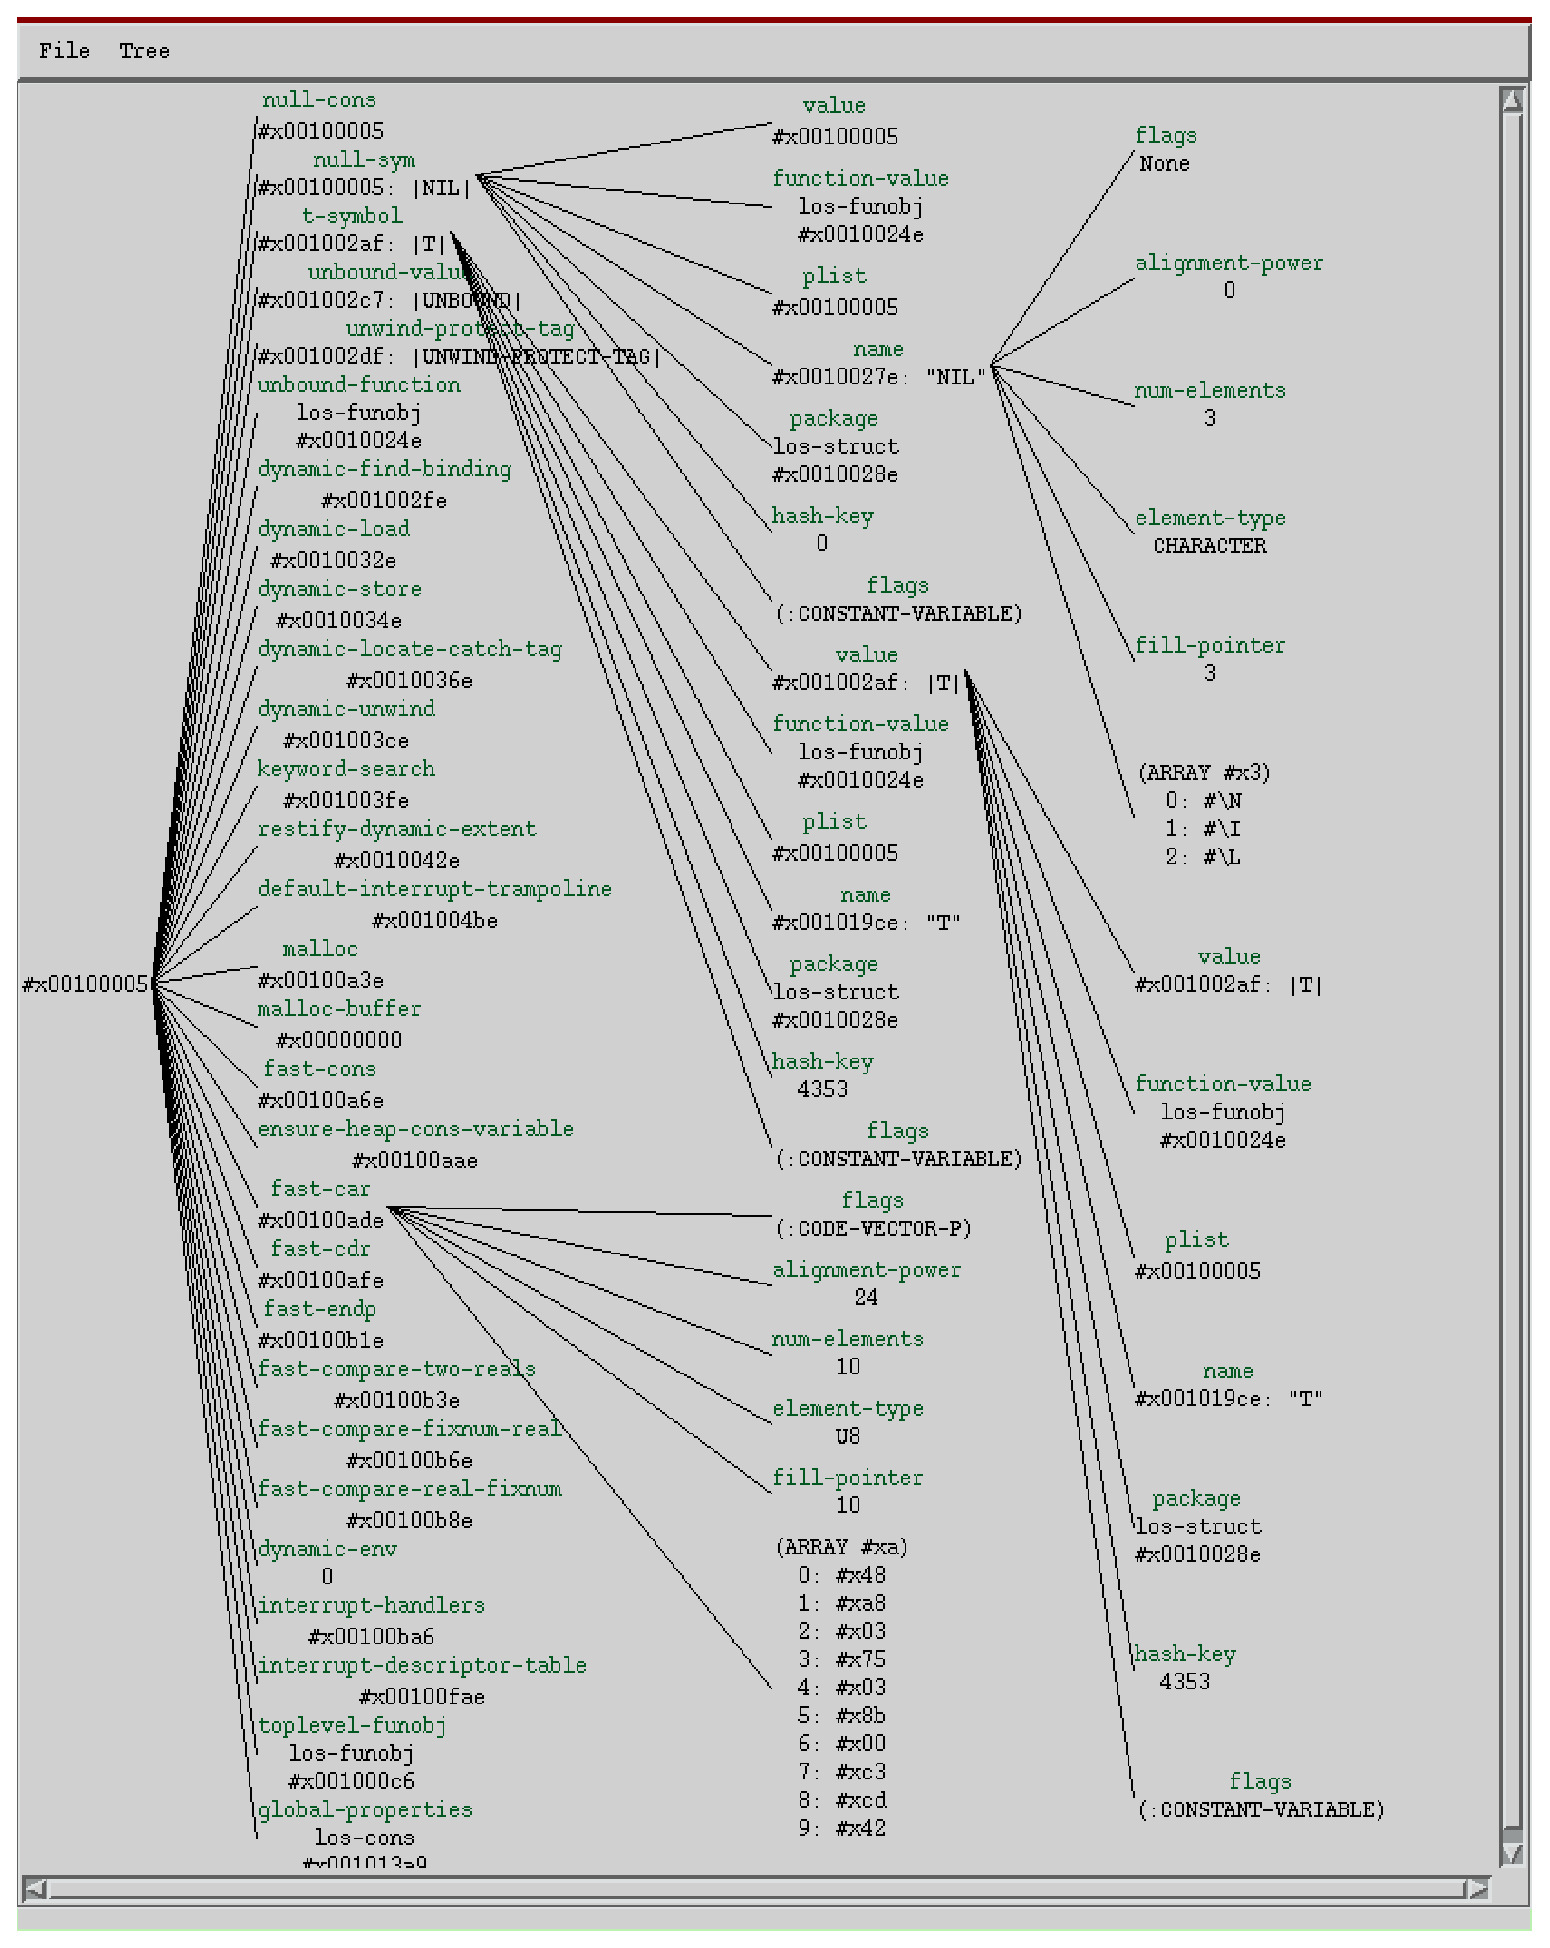
\includegraphics[width=\columnwidth]{browser}
  \caption{A screen-shot of the Movitz image browser tool. The root
    object to the left is the global ``run-time-context'', a.k.a\ the
    \clsym{nil} object.}
  \label{fig:browser}
\end{figure}

\subsection{Bochs emulator interface}

As previously mentioned, one of the image implementations interfaces a
running Bochs emulator, using the Unix procfs IPC mechanism. In
addition to providing access to the emulated address space, the entire
state of the emulated CPU is also made available. This enables for
example the developer to obtain a stack-trace of the running program.
This has proved to be a valuable debugging tool.


\section{Summary}
\label{sec:summary}

We have introduced the Movitz system, and described some of its most
important concepts, some technical details, and some of its current
shortcomings with respect to the Common Lisp standard.

Figure~\ref{fig:screenshot} shows a screen-shot of the Bochs PC
emulator running a Movitz image. The image has just been booted (the
minus signs in parens are the boot-loaders progress indicator), and a
short interactive session showing off some of Movitz' features is
displayed.

\begin{figure}[htbp]
  \vspace{2cm}
  \centering
  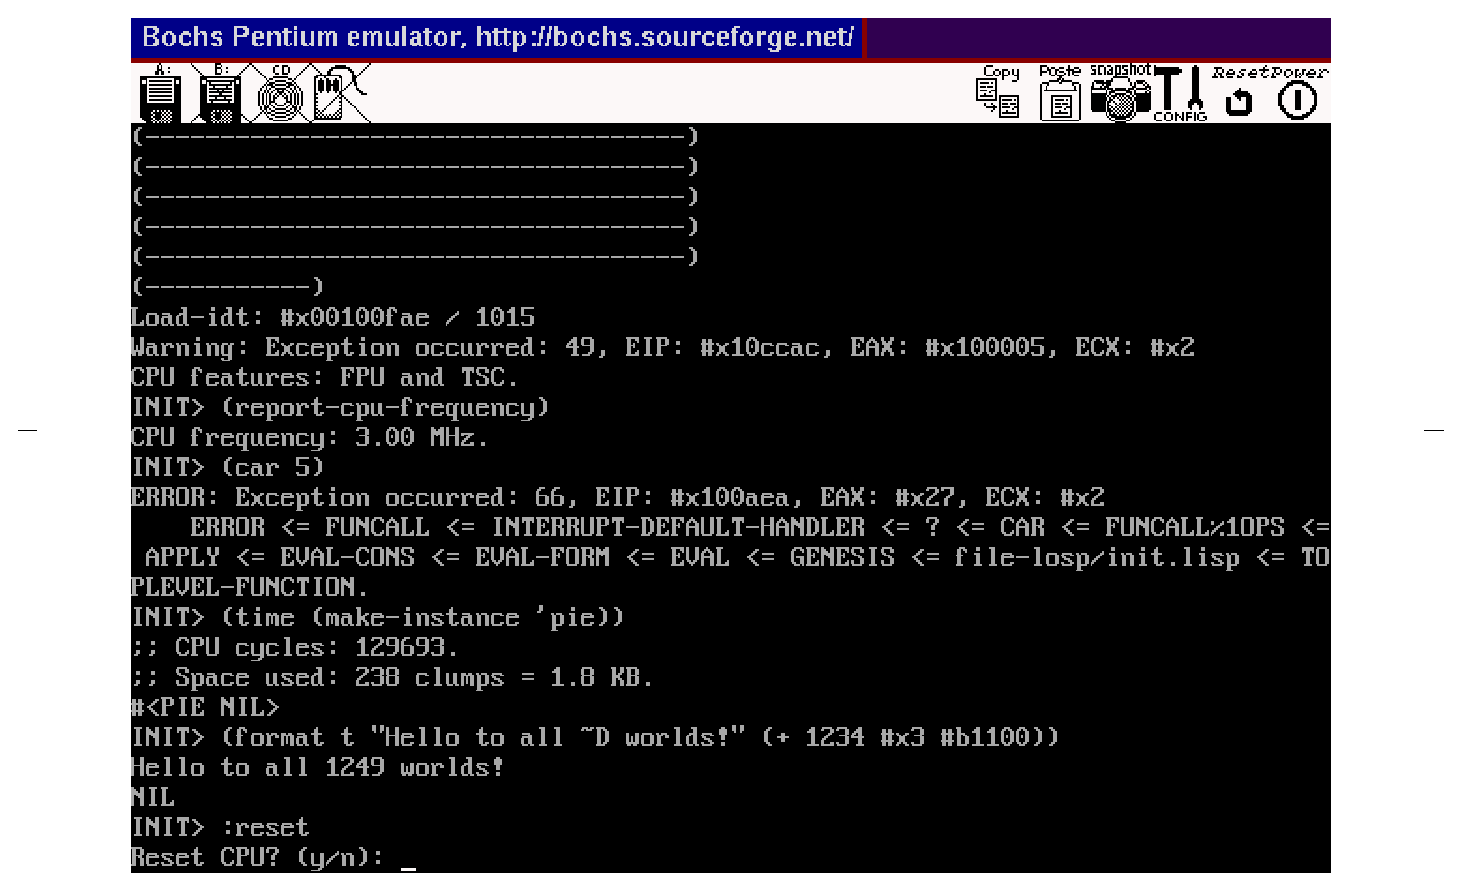
\includegraphics[width=\columnwidth]{screenshot}
  \caption{A screen-shot of Bochs running Movitz.}
  \label{fig:screenshot}
\end{figure}



\newpage

{\small\tableofcontents}

\newpage

\printindex[sym]


\end{document}

